\section{Access-control design}
\label{sec:design}

\subsection{Deployment structure and threat model}

The deployment has three tiers, shown in Figure~\ref{fig:architecture}. ESP32-WROOM-32 sensor nodes (dual-core Xtensa LX6 at 240\,MHz, 520\,kB SRAM) sample soil and environmental data, sign each reading with an Ed25519 key held in one-time-programmable eFuse, and transmit over LoRa. Raspberry Pi 4B zone gateways (quad-core Cortex-A72, 4\,GB LPDDR4, TPM 2.0) receive those payloads, verify signatures, endorse Fabric transactions and cache policy decisions locally. A Fabric network of \Gateways{} peers, one per zone, three Raft orderers and CouchDB 3.2 for world state maintains the ledger. Gateways interconnect over a BATMAN-adv mesh \citep{neumann2008batman} that reroutes around individual gateway failures and carries Fabric gossip and certificate revocation list (CRL) traffic between zones.

\begin{figure}[H]
\centering
\begin{tikzpicture}[every node/.style={font=\footnotesize}, node distance=0.75cm and 0.75cm,
    tier/.style={draw, rounded corners, thick, text width=8.6cm, align=center, inner sep=6pt}]
  \node[tier] (sensor) {\textbf{SENSOR TIER}\\\Sensors{} ESP32-WROOM-32 nodes (Ed25519 in eFuse, CRT residue transmission)};
  \node[tier, below=of sensor] (gateway) {\textbf{GATEWAY TIER}\\\Gateways{} zone gateways (Raspberry Pi 4B + TPM), BATMAN-adv mesh};
  \node[tier, below=of gateway] (fabric) {\textbf{FABRIC NETWORK}\\\Gateways{} peers (one per zone), 3 Raft orderers ($f{=}1$), CouchDB 3.2 world state, Fabric CA + CRL, HRBAC chaincode};
  \node[tier, below=of fabric] (stake) {\textbf{STAKEHOLDERS}\\Farmer/Admin, Agronomist, Certifier, Supply chain};
  \draw[->] (sensor) -- node[right] {LoRa} (gateway);
  \draw[->] (gateway) -- node[right] {Fabric gateway / peer} (fabric);
  \draw[->] (fabric) -- node[right] {zone-scoped queries and audit} (stake);
\end{tikzpicture}
\caption{Deployment architecture. Sensors reach the ledger only through their zone gateway, which is also their registration authority during enrollment. Zone membership is carried in the device certificate and re-checked by chaincode on every transaction.}
\label{fig:architecture}
\end{figure}

Following the permissioned-blockchain model in which every participant is credentialed \citep{androulaki2018hyperledger}, orderers and the certificate authority are operated by vetted institutional entities and treated as non-malicious; Raft's $2f{+}1$ crash-fault tolerance \citep{ongaro2014search} means the three-node cluster survives one orderer failure but not a reachable orderer behaving maliciously, a boundary Byzantine-tolerant ordering \citep{yin2019hotstuff,castro1999practical,hyperledger2025v3} would widen at higher consensus cost. Sensors, client devices and every wireless channel are treated as potentially compromised; physical tampering and side-channel extraction against cryptographic accelerators sit outside the evaluated scope (Section~\ref{sec:discussion}).

The design and the evaluation below distinguish six properties: authentication, authorization, integrity, freshness, auditability and availability. The deployment gives usable evidence about authorization (Section~\ref{sec:results-security}), auditability (every decision writes an audit entry, Section~\ref{sec:implementation}) and availability (Section~\ref{sec:availability}); it does not give usable evidence about authentication or integrity of sensor readings, because the signature path meant to bind a reading to its sensor did not function (Section~\ref{sec:sig-audit}), and freshness is architectural (nonce checking) rather than measured against an adaptive adversary.

\subsection{Role hierarchy}
\label{sec:role-hierarchy}

Following the treatment of hierarchical role administration in ARBAC97 \citep{sandhu1999arbac97}, a partial order $\preceq$ over the role set $R$ defines inheritance, with $r_i \preceq r_j$ iff $\mathrm{perm}(r_i) \subseteq \mathrm{perm}(r_j)$. The deployed hierarchy, reproduced in Figure~\ref{fig:hierarchy} directly from \texttt{chaincode/hrbac/roles.go}, is a human chain and a separate device chain, both below Admin:
\begin{align}
\text{SupplyChain} &\preceq \text{Certifier} \preceq \text{Agronomist} \preceq \text{Farmer} \preceq \text{Admin} \\
\text{Sensor} &\preceq \text{Gateway} \preceq \text{Admin}
\end{align}

\begin{figure}[H]
\centering
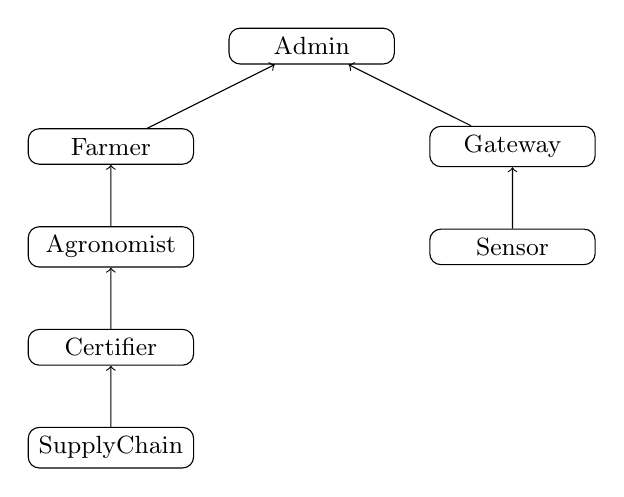
\begin{tikzpicture}[scale=0.85, every node/.style={draw, rounded corners, font=\small, minimum width=2.1cm, align=center}]
  \node (admin) at (5,4.5) {Admin};
  \node (farmer) at (2,3) {Farmer};
  \node (gateway) at (8,3) {Gateway};
  \node (agro) at (2,1.5) {Agronomist};
  \node (sensor) at (8,1.5) {Sensor};
  \node (cert) at (2,0) {Certifier};
  \node (supply) at (2,-1.5) {SupplyChain};
  \draw[->] (farmer) -- (admin);
  \draw[->] (gateway) -- (admin);
  \draw[->] (agro) -- (farmer);
  \draw[->] (sensor) -- (gateway);
  \draw[->] (cert) -- (agro);
  \draw[->] (supply) -- (cert);
\end{tikzpicture}
\caption{Seven-role hierarchy as deployed. Arrows point from a role to one that inherits its permissions, as implemented in \texttt{roles.go}. Certifier sits inside the human inheritance chain, so Agronomist and Farmer also inherit \texttt{ReadAudit} (Section~\ref{sec:audit-policy}).}
\label{fig:hierarchy}
\end{figure}

Separating auditors from operational staff is the requirement that motivated the model: an auditor should read compliance evidence without inheriting the agronomic permissions a farm treats as proprietary. Placing Certifier inside the human chain rather than beside it defeats that: Agronomist and Farmer inherit Certifier's permissions, including \texttt{ReadAudit}, so the deployment did not confine audit-log access to auditors. We verified this directly against \texttt{chaincode/hrbac/roles.go} (Section~\ref{sec:audit-policy}) rather than take it on the earlier draft's word; Table~\ref{tab:policy-table} gives the rows where intended, deployed and (specified, not implemented -- Section~\ref{sec:corrected-absent}) corrected policy disagree.

\begin{table}[H]
\centering
\caption{Permission grants where the intended design, the deployed chaincode and the specified correction disagree. Intended is independent requirements prose (Section~\ref{sec:role-hierarchy}), not derived from any code; Deployed is generated from \texttt{chaincode/hrbac/roles.go} (verified directly against the source in this repository). Corrected is a specified fix, arithmetically and logically checked by us, but \textbf{not implemented as a separate package in this repository} (Section~\ref{sec:corrected-absent}); every permission not listed here is identical across all three.}
\label{tab:policy-table}
\small
\begin{tabular}{llll}
\toprule
Permission & Role & Intended & Deployed \\
\midrule
ReadAudit & Agronomist & No & Yes \\
ReadAudit & Farmer & No & Yes \\
ReadZone & Certifier & No & Yes \\
ControlZone & Agronomist & No & Yes \\
\bottomrule
\end{tabular}

\smallskip
\footnotesize Specified correction: \texttt{ReadAudit} removed from Agronomist and Farmer's inherited set; \texttt{ReadZone} moved from Certifier to Agronomist's and Farmer's direct grants; \texttt{ControlZone} removed from Agronomist's direct grant and given to Farmer directly instead. This is the mapping used in \texttt{analysis/scripts/06\_security\_oracle.py}'s ``intended'' oracle (Section~\ref{sec:results-security}); it has not been implemented as running chaincode.
\end{table}

The effective permission set of user $u$ in a session is
\begin{equation}
\mathrm{eff}(u) = \bigcup_{r \in \mathrm{active}(u)} \bigcup_{r' \preceq r} pa(r'),
\end{equation}
where $pa(r)$ are the permissions assigned directly to $r$ and $\mathrm{active}(u)$ the non-expired roles held by $u$. An access request $(u, op, res, t)$ is granted iff
\begin{equation}
\exists r \in \mathrm{active}(u,t): (op,res) \in \mathrm{eff}(r) \wedge \big(\mathrm{zone}(u) = \mathrm{zone}(res) \vee czt(u,\mathrm{zone}(res),t)\big),
\end{equation}
where $czt(u,z,t)$ holds iff $u$ has a valid administrator-issued cross-zone token for $z$ at time $t$, and $\mathrm{active}(u,t) = \{r \mid \exists \mathrm{assign}(u,r,t_s,t_e): t_s \le t \le t_e\}$. The full effective-permission matrix this produces for all seven roles, generated from \texttt{roles.go} rather than transcribed, is in the supplementary material; Table~\ref{tab:policy-table} below gives only the rows that differ between what was intended, what was deployed, and the specified correction.

\subsection{Zone and temporal scoping}

Geographic farm regions (North, South, East, West) define the zone model, enforced at three independent points: certificate SAN field, gateway enrollment (own zone only), and chaincode's ASN.1-decoded zone check on every transaction, chosen over PEM-text matching because the latter is spoofable by an attacker who controls the subject field. Cross-zone tokens are administrator-issued and recorded immutably, so a temporary grant expires on its own rather than needing a reissued certificate. Temporal constraints run in two independent layers, the chaincode's \texttt{ExpiresAt} check against the Fabric transaction timestamp and the Fabric MSP's X.509 \texttt{NotAfter} validation, so a seasonal worker loses access at expiry without administrator action, recorded as a new audit entry; GPS-sourced gateway time, NTP fallback, sits comfortably inside the $\pm$5-minute enforcement window.

Two of the decision procedure's properties matter later: the work is bounded and independent of which operation was requested (hierarchy walked to depth at most three, zone check a single field comparison), the mechanism we would expect to produce similar costs across operations; and every path, including every denial, writes an audit entry, so \texttt{CheckAccess} is state-mutating and commits through ordering exactly as a sensor write does, with expired assignments revoked inside the same transaction that denies the request.

\subsection{Cascading enrollment}

An ESP32 cannot hold the TLS handshake state direct interaction with a certificate authority requires (mbedTLS on ESP-IDF needs roughly 70\,kB of heap against a 520\,kB SRAM budget \citep{raza2013lithe}), so registration authority moves down the tier structure in three stages: administrator credentials, then gateway registration with the private key in TPM 2.0, then sensor enrollment with the gateway as local registration authority. The sensor's key is generated on-device and never transmitted, so compromising a gateway does not yield it, and re-provisioning a lost key needs physical access, since eFuse programming is irreversible -- but the key is not read-protected: software signing copies it from eFuse into RAM each time, and setting the read-disable bit would break signing outright on this ESP32, which has no hardware Ed25519 engine. Read protection needs a different part (the ESP32-S3's HMAC and digital-signature peripherals); the eFuse here gives durability against reflashing, not extraction resistance against code running on the device, and Section~\ref{sec:discussion} counts key extraction by an attacker with code execution as residual risk.
